\section{Introduction}
\label{sec_opportunistic_intro}
	
	%\ac{MU-MIMO} is a transmission technique that enables a multi-antenna transmitter to transmit multiple, parallel data streams to distinct user nodes.
	%By pre-coding the data streams concurrently through a coherent antenna array, a transmitter can increase its spectral efficiency and overall downlink system capacity.  
	%Closed-loop \ac{MU-MIMO} transmissions first require a transmitter to measure the channel between itself and its receivers (a process known as channel sounding) before transmitting concurrent data streams to the receivers.
	%This direct measurement of \ac{CSI} adds considerable protocol overhead and must occur more often in time-varying channel environments since the beam-formed transmission is sensitive to channel variation.
	%A more temporally-correlated channel would allow a \ac{MU-MIMO} system to reduce \ac{CSI}-estimation frequency and improve the accuracy of this estimate for longer lag times.
	
		\ac{MU-MIMO} is a wireless channel coding technique that enables an \ac{AP} equipped with multiple antennas to transmit \textit{simultaneous} data streams to separate \acp{STA}, leveraging spatial diversity to scale data rates with the number of transmit antennas.
	For an \ac{AP} to use this technique, it must first estimate the \ac{CSIT} between each of its transmit antennas and each receiving antenna through a method termed \textit{channel sounding}.
	The estimated \ac{CSIT} is then	used to compute precoding weights for the multi-stream transmitter.
\ac{CSIT} can also be used for resource allocation, such as user grouping \cite{mao2012sus} and inter-cell interference mitigation \cite{rahman2010intercell}.

	IEEE 802.11af is a standard amendment for Wi-Fi to operate in unused UHF \ac{TVWS} channels \cite{flores2013af}.
	The standard can also employ MU-MIMO features of IEEE 802.11ac \cite{std11ac}: here, explicit \ac{CSIT} is obtained at the \ac{AP} by first transmitting a sounding packet from the \ac{AP} to the \ac{STA}, then having each \ac{STA} transmit the measured \ac{CSI} to the \ac{AP} as a control frame \cite{std11af}.
	Unfortunately, the transmission overhead required for \ac{CSIT} estimation increases with the number of transmit antennas at the \ac{AP}, $M$, and the number of aggregate \ac{STA} antennas, $K$, and recent results have shown that this overhead can severely decrease the achievable throughput gains \cite{xie2013adaptive, bejarano2014mute}.
	
	%In this final chapter, we explore elimination of explicit channel sounding altogether via purely \textit{opportunistic} channel sounding in which \ac{CSIT} is implicitly estimated from each received \textit{uplink} transmission, whether a data or control frame. 

	In this final chapter, we leverage our results to design a new random-access technique called Opportunistic Implicit Channel Sounding in order to support throughput scaling of 802.11 multi-user random access as the number of base station antennas continues to grow.
	
	%#######################################################
\subsection{Implicit vs. Explicit Channel Sounding}
\label{sec_im_vs_exp}

 Implicit beamforming relies on the assumption that the physical channel between the transmitter and receiver is reciprocal in nature so that estimating \ac{CSI} in the downlink direction is equivalent to estimating \ac{CSI} in the uplink direction and vice versa.
 Accurate array reciprocity calibration has been demonstrated \cite{shepard2012argos}, and \cite{guillaud2013reciprocity} has experimentally demonstrated equivalent mutual information between downlink and uplink channel estimates utilizing transceiver hardware similar to our own.
 Therefore, we assume that uplink channel estimation is sufficient to estimate the downlink channel for our purposes, and we assume that all new \acp{AP} will have the capability to perform reciprocity calibration and provide implicit channel estimation.
 
 The benefits of implicit channel sounding vary based on node/environment mobility as well as the protocol and radio configuration utilized.
For example, if the wireless channel varies rapidly due to high mobility, frequent channel sounding, whether implicit or explicit, will be required to obtain accurate \ac{CSIT}.
 Per-packet channel sounding mechanisms that incur protocol overhead, such as the multi-user implicit sounding mechanism analyzed in \cite{lou2013comparison} may be required to ensure that channel estimates are accurate in such environments.

However, in the case where the wireless channel remains coherent for long periods of time, for example, due to limited or lack of mobility, then it becomes possible to rely on previously collected \ac{CSI} for current \ac{MU-MIMO} transmissions \cite{bejarano2014mute, xie2013adaptive}.
Practically, such environments exist in wireless networks utilizing sub-GHz carrier frequencies, for instance \ac{TVWS} networks \cite{anand2014case}, as well as certain fixed Wi-Fi networks.

% 
\section{Opportunistic Channel Estimation for Implicit MU-MIMO}
\label{sec_opportunistic}

%\rgnote{This is where the setup and simulation work for [ITC 2016] goes. I've copied the paper intro--it needs to be made into a section intro.}
This approach exploits a key property of UHF bands: they can be highly stable on the order of 100~ms while maintaining high multi-user diversity \cite{anand2014case}.
Thus, the opportunistic policy eliminates \ac{CSIT} sounding overhead if the channel remains
sufficiently unchanged between uplink transmissions.
Otherwise, the AP can fall back to active channel sounding modes in the case of rapid channel variation or insufficient uplink traffic.  
	
We show that opportunistic sounding is beneficial in four operating regimes in which: \emph{(i)} channel conditions are sufficiently stable such that beamforming error due to obtaining \ac{CSIT} from a prior uplink transmission is negligible; \emph{(ii)} legacy 802.11 \acp{STA} cannot respond to beamforming requests and otherwise could not leverage full spatial diversity; \emph{(iii)} the number of spatial streams grows such that even implicit channel estimation generates significant overhead; and \emph{(iv)} the \ac{MCS} is sufficiently high that any wasted airtime due to channel sounding overhead imposes a high relative cost.
Scenario \textit{(ii)} is of particular interest because it enables new 802.11 \acp{AP} with multi-user capabilities to operate in spectral-efficient multi-user modes with legacy 802.11 equipment that does not otherwise support multi-user modes.

To explore the key performance factors of opportunistic sounding, we design and manufacture a custom MIMO \ac{SDR} front-end for the WARPv3 \ac{SDR} platform \cite{warpProject}.
This platform enables the first characterization of mobile multi-user UHF channels, enabling
evaluation of opportunistic sounding even in the presence of \ac{STA} or environmental mobility.
The design simplifies high-power UHF-band 8x8 MIMO experiments and improves synchronous clocking over previous \ac{SDR} testbeds.
In addition to implementation of custom \ac{SDR} hardware, we modify a novel \ac{SDR} channel sounding framework designed for high-speed mobile implicit multi-user channel measurements \cite{shepard2015faros} and port the framework to operate on our UHF equipment.
	
We find that fixed wireless nodes utilizing UHF spectrum exhibit long-term stable \ac{CSI} under environmental and static mobility scenarios.
Consequently, we find that with a low number of spatial streams, performance of both active and opportunistic implicit sounding policies significantly exceeds that of the current 802.11af protocol due to the reduced overhead of collecting \ac{CSI}, even when taking into account the measured beamforming inefficiency of using delayed \ac{CSIT}.
We further extend our analysis to show that opportunistic implicit sounding with more spatial streams yields increasing benefits, enabling future systems with many more antennas than the current maximum of eight in commodity \acp{AP}.
	
%####################################################################################
\subsection{Opportunistic \ac{CSIT} Collection}
\label{sec:wurcProtocol}

\begin{figure*}[t] % Channel Sounding Types
\centering
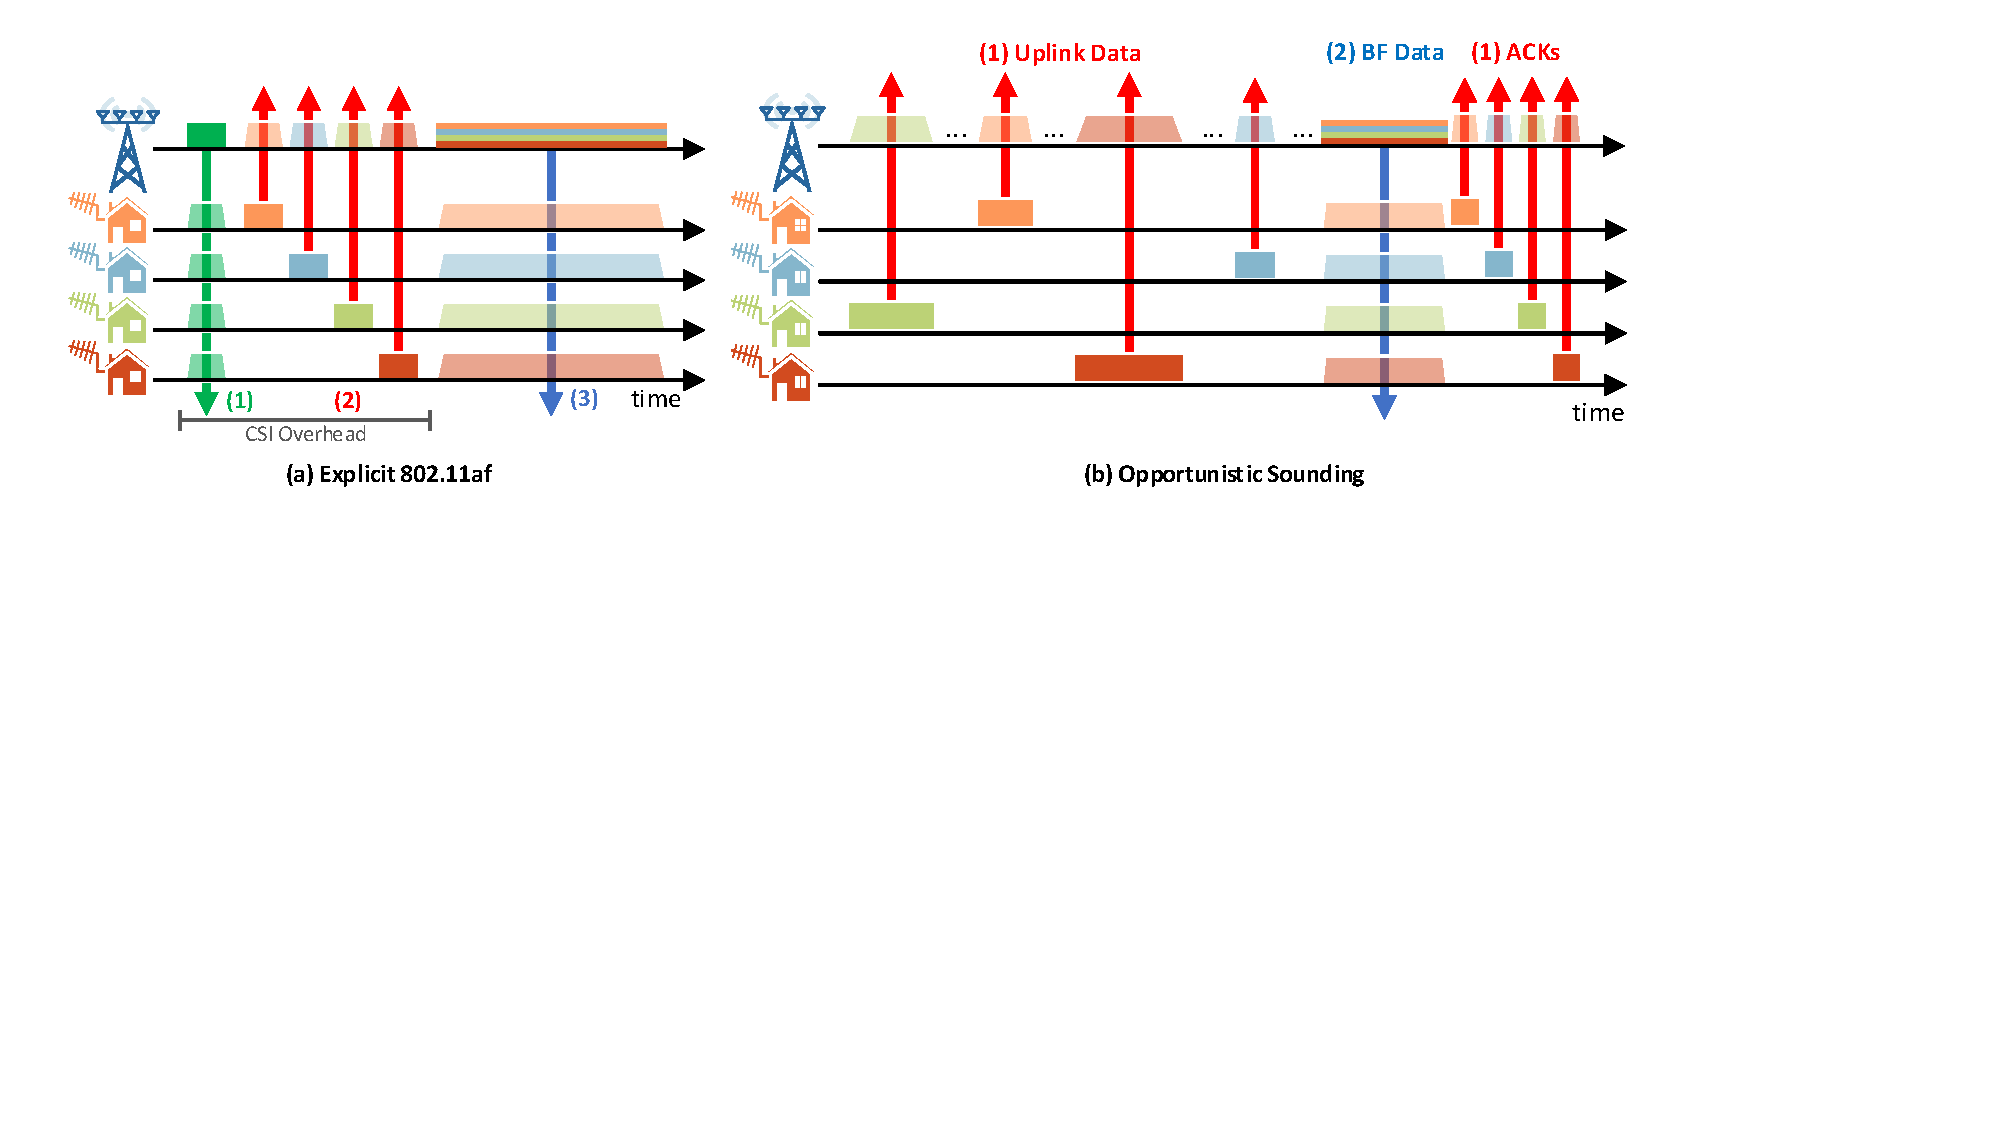
\includegraphics[width=1\textwidth]{figs/protocol/opportunistic_diagram.pdf}
\caption{Time diagram of the considered types of channel sounding. 802.11af polling packets are not included in the explicit sounding diagram.}
\label{fig:soundingDiagrams}
\end{figure*}

In this section, we propose a new approach to collecting \ac{CSIT} in 802.11af networks that avoids the overhead of \ac{MU-MIMO} channel sounding altogether by relying on the opportunistic reception of implicit \ac{CSI} for regular network traffic.

 Fig.~\ref{fig:soundingDiagrams}a diagrams explicit channel sounding, where first the downlink channel is estimated and then the channel estimates are fed back as data packets before each multi-user downlink transmission.
 This method, with additional polling and channel reservation overhead, is the version currently used in 802.11af \cite{std11af}.
 Explicit beamforming overhead scales as $\mathcal{O}(M\cdot K)$.

 A proposed implicit sounding method \cite{lou2013comparison} that transmits staggered \acp{NDP} in the uplink direction allowing implicit downlink channel estimation following a multi-user trigger from the \ac{AP}.
 Its timeline is similar to that of Fig.~\ref{fig:soundingDiagrams}a, but instead the uplink packets are short \acp{NDP} rather than \ac{CBFR} packets, and polling is avoided.
 Implicit channel estimation overhead is significantly reduced from the explicit case since no \ac{CBFR} polling or uplink payload is required before the downlink transmission.
 Implicit beamforming overhead scales as $\mathcal{O}(K)$ since all \ac{AP} antennas are sounded simultaneously and is key for scaling $M$, the number of \ac{AP} antennas.

 Fig.~\ref{fig:soundingDiagrams}b displays our proposed \textit{opportunistic} implicit sounding method that estimates the downlink channel implicitly from uplink data transmissions and utilizes that channel estimate for \ac{MUBF} so long as it remains ``fresh.''
 \ac{ACK} packets from a successful downlink transmission can also refresh \ac{CSIT} implicitly.
 Opportunistic implicit beamforming overhead scales as $\mathcal{O}(1)$ since no sounding overhead is injected to sound active \acp{STA}.

 Given that the UHF channels for 802.11af networks can remain stable for relatively long periods of time, we target to avoid channel sounding altogether and rely on standard PLCP preambles \cite{std11af} in overheard uplink transmissions to estimate the downlink channel since that estimate will remain valid over multiple packet timescales.

 The key strategy for opportunistic sounding is as follows: when historical implicit CSI is available and ``fresh,'' the \ac{AP} forms user groups and calculates precoding weights for the optimal multi-user transmission group determined by the MAC scheduler.
 We utilize two methods when implicit \ac{CSI} is unavailable or stale for a particular \ac{STA}: 1) a single downlink frame for the stale \ac{STA} is de-queued and transmitted by the AP using MISO omni-directional transmission; the subsequent \ac{ACK} will then provide an update of implicit \ac{CSI} for that \ac{STA}; or 2) alternately, the \ac{AP} could fall back to legacy implicit sounding methods, e.g., \cite{lou2013comparison}, if no traffic is available.

 In order to determine the feasibility of such an opportunistic sounding policy in 802.11af systems and explore the possible throughput gains, we measure a series of indoor and outdoor multi-user channel traces and perform protocol analysis to understand policy tradeoffs for opportunistic \ac{CSIT}.
	
\subsection{Performance of Proposed 802.11af Sounding Alternatives}
\label{sec:protocolSimulation}
%\eknote{the subsection title shold focus on the issue vs. the tool (sim vs. OTA}
%\eknote{are these trace-driven simulations?}

 In this section, we investigate the protocol gains available from an opportunistic \ac{CSIT} system with regard to various MAC-layer parameters.
 We also compare performance against an implicit sounding policy adapted from 802.11n standard proposals for multi-user operation \cite{lou2013comparison}. 
 %Although UHF radio spectrum is highly valuable due to its licensing structure and superior propagation characteristics, the fragmentation of UHF spectrum into many small 6~MHz channels and the relatively large antenna apertures of UHF bands means that scaling capacity with \ac{MU-MIMO} is critical \cite{anand2014case} and therefore reducing \ac{CSIT} overhead is very important.

 The 802.11af standard attempts to amortize explicit sounding overhead by transmitting aggregated data frames, however the efficiency of this approach depends on the number of frames actually available to aggregate.
 We analyze the protocol performance of a \ac{MU-MIMO} system with various channel sounding policies and with varying packet aggregation values in order to emulate both best and worst case scenarios.
 %Since our proposed opportunistic system will discard historical \ac{CSIT} when it is determined to be stale, the stale channel must be resounded either explicitly or via a unicast transmission to that \ac{STA} resulting in an ACK that can then be used to refresh implicit \ac{CSIT}.

 %In the worst-case transmission scenario, the system would have no fresh \ac{CSIT} and performance would revert to the implicit/explicit curves or the opportunistic \ac{AP} would send unicast transmissions to all \acp{AP} before sending multi-user data.
 
 We set the single frame size to 1500~bytes, the largest regular Ethernet frame size and the best case for \ac{CSIT} overhead amortization before aggregation.
%\eknote{bytes or kB? frame aggregation would be the best case so should rephrase}
 We compare three different channel sounding policies:

\textbf{Explicit 802.11af.} This is the current standard operation of 802.11af \ac{MU-MIMO}. \ac{CSIT} overhead in this case is caused by the \ac{NDP} Announcement, the sounding \ac{NDP}, and the sequence of polls and \ac{CBFR} responses from all 802.11af \acp{STA} before each downlink transmission \cite{std11af}.
 The upper and lower bounds on explicit performance are calculated with minimum and maximum feedback compression of the \ac{CBFR} payload, a highly vendor-specific implementation parameter.
 We assume no impairment on performance from feedback compression, and plot the median performance while indicating the bounds with a shaded red region.

 Although the 802.11af standard only supports up to 8 concurrent spatial streams, we assume that timing and protocol performance scales with the number of streams in order to provide a point of reference for scaling to large numbers of antennas.
We label this policy \textit{``Explicit 802.11af''} in the following plots.

%\eknote{I'm not in favor of calling anything 802.11af unless it IS 802.11af. there is no such thing as implicit
%11af and the reader might be confused (and might reject the paper and explain to you that you've misunderstood
%the standard and don't know how it works.}

\textbf{Implicit Proposal for 802.11af.} 
	In \cite{lou2013comparison}, the authors proposed an alternative  multi-user \ac{CSI} sounding protocol that avoids the lengthy \ac{CBFR} by estimating the channel implicitly with short \acp{NDP}.
	\ac{CSIT} overhead in this case comes from the \ac{NDP} Announcement and a staggered sequence of uplink \acp{NDP} that are used for implicit channel estimation before each multi-user transmission as proposed in \cite{lou2013comparison}.
	Since the channel is estimated implicitly, there are no levels of feedback compression to display.
	We label this policy \textit{``Implicit''} in the following plots.

\textbf{Opportunistic Proposal for 802.11af.}
	In this case, there is no \ac{CSIT} overhead to multi-user transmissions.
	We explore three regions of operation for an opportunistic \ac{AP}:
\begin{enumerate}
\item \textit{``Opportunistic.''} The best-case performance assuming all \ac{CSIT} is available opportunistically and there is no beamforming penalty for using stale \ac{CSIT}. This is an upper bound on opportunistic performance since practically all \ac{CSIT} will have some error.

\item \textit{``Opportunistic with Bootstrap.''} An alternative fallback mode where at most one \ac{STA} has stale \ac{CSIT} and the \ac{AP} sends a single
%\eknote{do not use unicast here as it seems you are contrasting to multicast but you are actually contrasting to multi-user}
packet to that \ac{STA} before each multi-user transmission in order to implicitly refresh its \ac{CSIT}.
This can be viewed as a way of quickly bootstrapping opportunistic \ac{CSIT} to a \ac{STA} that previously was inactive.

\item \textit{``Opportunistic with Stale CSIT.''} A trace-driven lower bound on opportunistic performance based on our environmental measurement traces.
We assume that \ac{CSIT} is refreshed opportunistically every second.
According to our empirical results in Figure~\ref{fig_power_allocation}, this would result in less than 10\% reduction in achievable sum-rate in an environment with static \acp{STA}.
Thus, we reduce the throughput of the best-case opportunistic scenario by the requisite amount, presenting a more fair approximation of how an implemented opportunistic system might perform.
\end{enumerate}

 %If \textit{more} than one channel is stale, it is generally better to fall back on implicit channel sounding rather than to expend overhead in a unicast transmission to refresh opportunistic \ac{CSI}.
 %We ignore the increased per-\ac{STA} \ac{SINR} that would be achieved with a MISO transmission compared to a corresponding multi-user transmission and assume the underlying PHY rate remains the same.

 All \acp{ACK} are staggered as per the 802.11af specification.
 For tractability, transmissions are assumed to be successful, requiring no retransmissions, and only downlink data flows are considered.

%\rgnote{Question for reviewer: is the ``Opportunistic w/ Stale CSIT'' curve confusing?}

% Sounding 4x4 Policy
\subsection{Sounding Policy Performance: 4x4}
\label{sec:4x4_policy}
 
 In Fig.~\ref{fig:protosim_4x4}, we vary the multi-user frame aggregation number from $1$ to $64$ for the lowest (top) and highest (bottom) 802.11af \ac{MCS} in a $4\times 4$ system where all \acp{STA} have only a single antenna.

\begin{figure}[t] % FROZEN Simulation - 4x4  6 Mhz TVWS
\centering
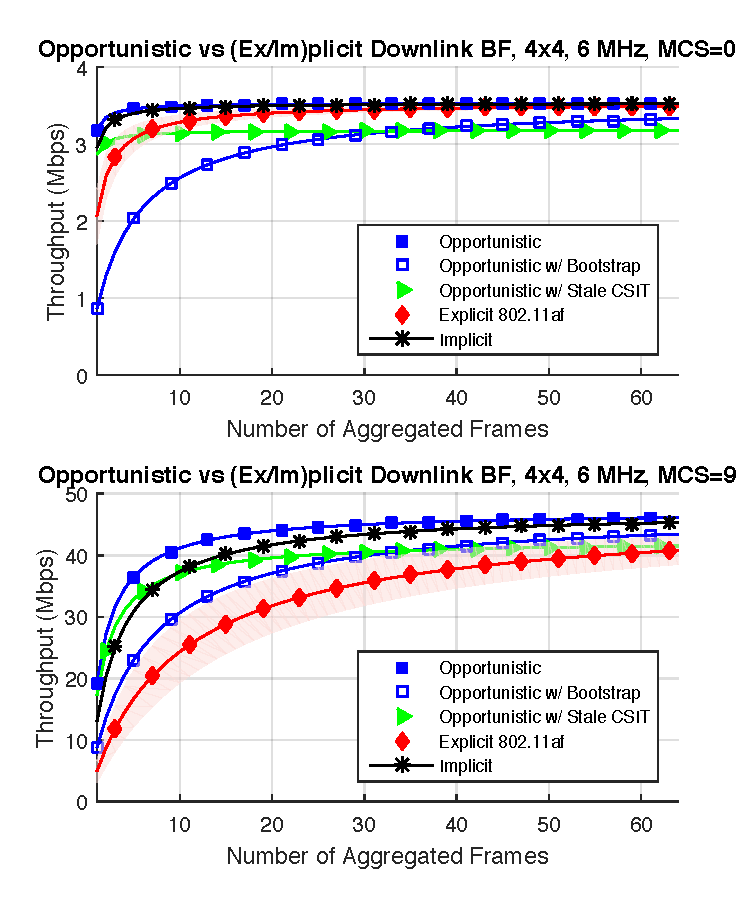
\includegraphics[width=0.7\linewidth]{./figs/protocol/tput_vs_agg_4x4_6mhz_im_mcs-0_crop}
\caption{Network throughput for a 4x4 802.11af system on a 6~MHz UHF channel. Base rate (top) and maximum \ac{MCS} (bottom).}
\label{fig:protosim_4x4}
\end{figure}

\begin{figure}[t] % FROZEN Simulation - 8x4  6 Mhz TVWS
\centering
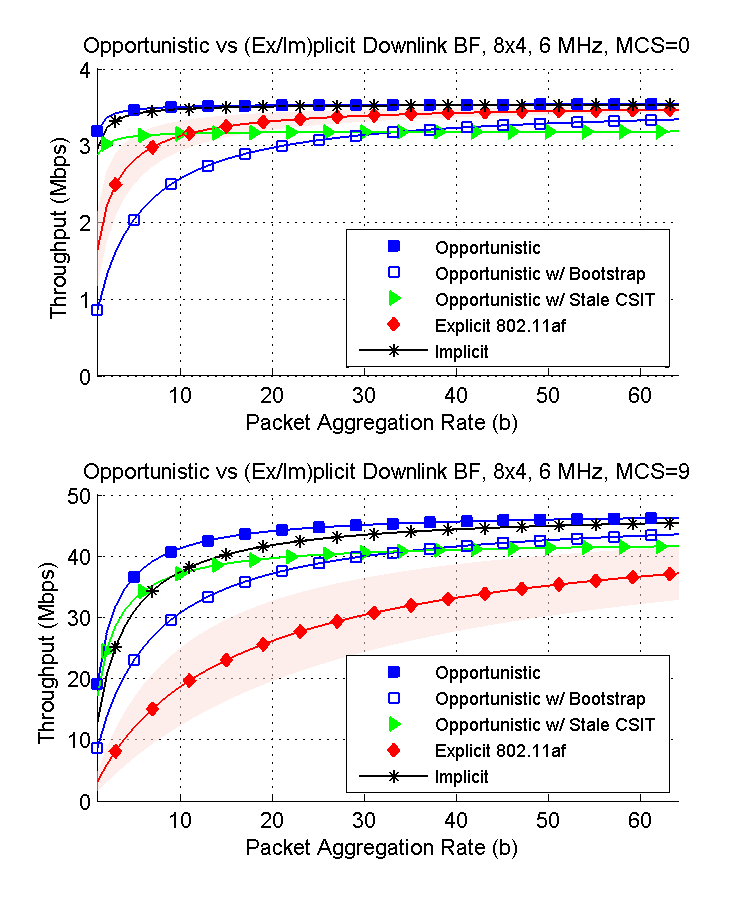
\includegraphics[width=0.7\linewidth]{./figs/protocol/tput_vs_agg_8x4_6mhz_im_mcs-0}
\caption{Network throughput for an 8x4 802.11af system on a 6~MHz UHF channel. Base rate (top) and maximum \ac{MCS} (bottom).}
\label{fig_protosim_8x8}
\end{figure}

\subsubsection{Effect of Frame Aggregation}
%\eknote{rough org. this is the basic X axis so it is awkward to first discuss and conclude about grphas without
%mentioning what the x axis is and then come back to the x axis. treat graphs completely with 4 steps one by one}
	Frame aggregation allows the cost of channel sounding to be amortized over large payloads. While we expect that increased aggregation will generally decrease the efficiency of channel sounding reduction protocols, it also determines crossover points in terms of protocol performance.
	
	At the lowest \ac{MCS} in the top plot of Fig.~\ref{fig:protosim_4x4} with no frame aggregation, there is a moderate performance gap between implicit channel sounding methods (opportunistic, implicit) and the current explicit 802.11af policy.
	An opportunistic sounding policy would increase throughput at best by 31\%, while an implicit sounding policy would increase throughput by 21\% over explicit 802.11af.
	However, as the aggregation rate increases, these alternatives rapidly converge. %around $b=10$, or 15~kB
	%\eknote{check this}
	%of aggregated payload data per-user.
	
%We observe that the proposed opportunistic bootstrapping mechanism performs poorly when operating at low \ac{MCS} since there is little benefit to transmitting a payload while sounding the stale \ac{STA} and it is always better to transmit a short explicit sounding handshake.\csnote{todo:improve readability}

		%When operating at low \ac{MCS}, there is negligible benefit to using opportunistic sounding in the best case and significant penalties compared to alternatives on the order of 10\% when considering stale \ac{CSIT}.
	
\subsubsection{Effect of Modulation and Coding Scheme}
 In general, the lower the \ac{MCS} rate, the lower the relative overhead of sounding; thus the use of any particular sounding mechanism matters much less at low rates than high rates.
	
	At base rate, shown in Fig.~\ref{fig:protosim_4x4} (top), there is little advantage in opportunistic sounding, and our proposed bootstrapping method under-performs even explicit sounding.
	However, as the \ac{MCS} of the system increases, the relative cost of sounding overhead also increases since airtime becomes more valuable, potentially compensating for the stale \ac{CSIT} penalty.
	
	In Fig.~\ref{fig:protosim_4x4} (bottom), we show the same results for the maximum supported \ac{MCS}.
	802.11af sounding overhead is much more costly when the system could otherwise be operating at high \ac{MCS}, since \acp{CBFR}, polling packets, and \acp{ACK} are all sent at base rate for robustness.
	The large range in explicit 802.11af sounding performance (red region) stems from the fact that uncompressed \ac{CBFR} packets take a significant amount of airtime, resulting in very high overhead.
	At high \ac{MCS}, opportunistic sounding can improve throughput by 186\% and implicit sounding can improve by 94\% without frame aggregation.
	
	While opportunistic sounding with stale \ac{CSIT} is strictly better than explicit 802.11af up to 35 aggregated frames, it barely out-performs implicit sounding at low aggregation with fewer than $10$ frames and then performs significantly worse with higher frame aggregation.

%\eknote{again a conclusion without
%going through the figure. no description or analysis} in either implicit sounding policy since overhead incurs a relatively small penalty compared to the low \ac{MCS}.

%At the lowest \ac{MCS} in the top of Fig.~\ref{fig:protosim_4x4}, there is a severe difference in performance when only a few packets are available to be aggregated.


 %\eknote{no discussion of the VERY wide bounds at lower vs. higher aggregation rates and why they narrow}

	Therefore, we conclude that for a low number of spatial streams, opportunistic channel sounding has approximately equivalent performance compared to implicit channel sounding and potentially worse performance when considering beamforming error from stale \ac{CSIT}.
	However, both opportunistic and implicit channel sounding offer significant throughput gains over the current explicit 802.11af standard.
	
	The best usage scenario for opportunistic sounding in this regime is when implicit \ac{STA} cooperation is not possible, such as with current 802.11 devices.
	A system design that leverages this observation would utilize \textit{opportunistic} \ac{CSIT} when per-user downlink traffic queues are below 3-52~MB, depending on the current \ac{MCS}, and then revert to explicit sounding when queues exceed that size and sounding overhead can be sufficiently amortized.
	For legacy 802.11a/b/g/n devices that do not report any CSIT, only opportunistic \ac{CSIT} would be available and the decision is made between multi-user and single-user transmission modes only.

	 %We also conclude that even with low numbers of spatial streams, an implicit sounding policy can drastically increase the capacity of 802.11af systems, with negligible improvement for operation at low \ac{MCS}.
 %In high \ac{SINR} regimes with many short-lived flows, implicit channel sounding could significantly increase protocol throughput for 802.11af systems.

%\eknote{interesting subsection. needs the above structure/analysis changes} 
%\eknote{this seems to be one of the larger punchlines of the entire paper and it's buried at the very end.
%since implicit seems to do pretty well in Fig 10, the big gain seems to be when the entire system
%scales up. Given that, the paper sould really be ``Opportunistic Channel Sounding for Scaling
%to Massive MU-MIMO'' if this is a design paper. Otherwise, you're more agnostic to exp/implicit
%and opportunistic/not and the title would be more like
%``Implementation and Experimental Performance Evaluation of CSI Management Strategies on MU-MIMO
%Performance in UHF Bands''}

% Sounding 32x16 Policy
%\subsubsection{Sounding Policy Performance: 32x16}
\subsection{Scaling to 32x16}
\label{sec:scaling}

	At all \ac{MCS}, the challenge of efficiently using narrow bands of UHF radio spectrum is clear: system throughput is no more than 50~Mbps even with full 8x4 spatial diversity at the maximum \ac{MCS} (Figure~\ref{fig_protosim_8x8}).
	For this reason, we explore the possibility of leveraging additional spatial streams for UHF-band communications as a means of increasing spectral efficiency.

 Given the potential for large-scale 802.11af system installations to establish long-range point-to-multi-point networks and the need to support high throughput over narrow UHF channels, we extend our beamforming protocol analysis to a $32\times16$ system in Figure~\ref{fig:protosim_32x16}.
 Previous work on many-antenna \ac{MU-MIMO} systems has proposed implicit channel sounding as a means to avoid protocol collapse as the number of antennas at the \ac{AP} grows \cite{shepard2012argos}.
 Our results in Figure~\ref{fig:meas_corr} and Figure~\ref{fig_power_allocation} indicate that the \ac{CSI} of stationary \acp{STA} in both indoor and outdoor environments remain constant for long periods of time, which supports the possibility of using opportunistic sounding policies to increase system throughput even further.

	In all cases with a large number of spatial streams, explicit channel sounding suffers severely from protocol congestion due to the high number of spatial streams and amount of explicit data that is transmitted to the \ac{AP} to report \ac{CSI}.
	
	\begin{figure}[th!] % FROZEN Simulation - 32x16 6 Mhz TVWS
\centering
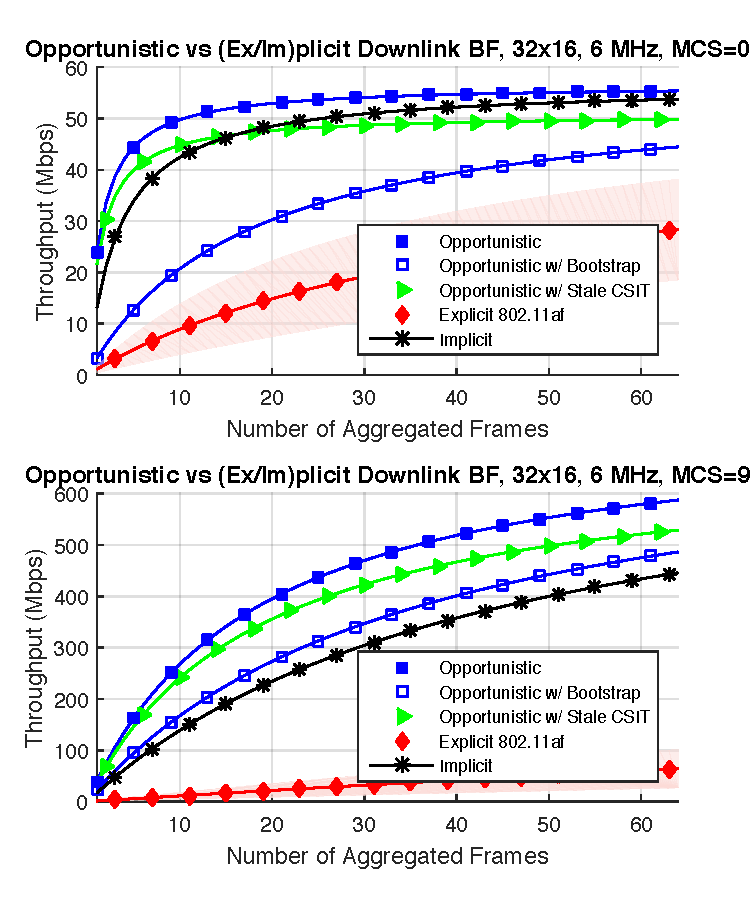
\includegraphics[width=0.7\linewidth]{./figs/protocol/tput_vs_agg_32x16_6mhz_im_mcs-0_crop}
%\vspace{-6mm}
\caption{Network throughput for a 32x16 802.11af system on a 6~MHz UHF channel.}
\label{fig:protosim_32x16}
\end{figure}

	In Figure~\ref{fig:protosim_32x16} (top), we see that for low \ac{MCS} rates and frame aggregation below $18$ frames, opportunistic sounding with stale \ac{CSIT} out-performs even implicit sounding, given the number of \acp{STA} involved in each transmission.
	
	In Figure~\ref{fig:protosim_32x16} (bottom) at the maximum supported \ac{MCS}, strict relationships emerge between the sounding policies, since \ac{CSIT} overhead dominates any other effects at this scale.
	When channel sounding becomes extremely expensive, the use of opportunistic \ac{CSIT} is able to offer significant throughput gains over implicit sounding, ranging from 112\% with no frame aggregation, to 18\% at maximum aggregation, even when considering the penalty from stale \ac{CSIT}.
	Explicit sounding should be avoided altogether.

	It is clear from Figure~\ref{fig:protosim_32x16} that network throughput for a 6~MHz channel can be significant in high-\ac{SNR} environments where high modulation rates can be achieved.
	When channel bonding multiple 6~MHz \ac{TVWS} channels, it is clear that multi-gigabit network throughput is achieveable with large-scale multi-user beamforming systems using implicit beamforming, and further increased in fixed deployments by using opportunistic beamforming.

%% Sounding 8x8 Wi-Fi Policy
%\subsubsection{Comparison with 802.11ac: 8x8}
%\label{sec:wifi_policy}
%
 %Until now, we have focused on the performance of opportunistic resounding 
%
 %The analysis in \S~\ref{sec:4x4_policy} and \S~\ref{sec:scaling} indicate that the efficiency of opportunistic channel sounding increases as the relative rate of the payload increases relative to the channel overhead.
 %This would suggest that high-rate 802.11ac systems with high channel bandwidth would benefit greatly from implicit modes of channel sounding.
 %On the other hand, the increase channel coherence time of 2.4 and 5.8~GHz channels could potentially prevent the use of opportunistic channel sounding.
 %In order to 
%
%\begin{figure}[h] % FROZEN Simulation -8x8 40 MHz Wi-Fi
%\centering
%\includegraphics[width=1\linewidth]{./figs/tput_vs_agg_8x8_40mhz_mcs-0.pdf}
%\caption{Network throughput for a 8x8 802.11ac system on a 40~MHz Wi-Fi channel.}
%\label{fig:protosim_8x8}
%\end{figure}
 
% Opportunistic Sounding Conclusion
\section{Discussion and Conclusion}
\label{sec_protocol_conclusion}
 
 In order to scale the capacity of \ac{MU-MIMO} beamforming systems, it is important to address the problem of \ac{CSIT} overhead, particularly in 802.11af systems with potentially limited system bandwidth.

 In this work, we developed a new \ac{SDR} system specifically for UHF-band \ac{MU-MIMO} that allowed us to gather the first mobile multi-user channel traces in the UHF band, which can be found in reference \cite{shepard2016understanding}.
	Based on our analysis of beamforming capacity with stale \ac{CSIT} in Section~\ref{sec:uhf_outdoor_results}, we showed large S-T intervals can be tolerated in UHF frequency bands, enabling the gathering of \ac{CSIT} purely opportunistically and enabling multi-user transmissions with legacy 802.11 equipment that can not provide \ac{CBFR} reports.

 We compared three different channel sounding policies and showed that for a small number of spatial streams, significant throughput gains are available with either of the implicit sounding policies, though the penalty of using stale \ac{CSIT} would encourage the use of implicit sounding rather than opportunistic sounding, if available.
 However, as the number of spatial streams increases, the overhead of even implicit beamforming begins to become a bottleneck on 802.11af performance and opportunistic channel sounding becomes much more beneficial when the nodes are stationary.
	%Given the limitations of our hardware platform, we were not able to experimentally validate the performance of 
%\csnote{removed `as APs and STAs grow in complexity' since it was very awkward and confusing.  perhaps we should say something about next-generation/emerging/many-antenna though} \rgnote{no room! :(}
%\csnote{I would try to make the conclusion sound more impressive 'up to XX fold gains'}

